\documentclass[a4paper,pdftex]{article}

\usepackage{array}
%\usepackage{mathtools}
\usepackage{hopsantut}
\usepackage{listings}
\usepackage{todonotes}
\usepackage[fleqn]{amsmath}
\usepackage{tikz}

\hypersetup{pdfauthor={Robert Braun and Peter Nordin}, pdftitle={Hopsan Tutorial - Writing Advanced Components}, pdfsubject={Hopsan Tutorial}}

\lstset{ %
  numbers			=	left,
  numberstyle		=	\scriptsize, % the style that is used for the line-numbers
  backgroundcolor	=\color{yellow!10}
}

\begin{document}
\maketitle{Writing Advanced Components}

\section*{Introduction}
This tutorial is a continuation of the \textit{Writing Component Libraries} tutorial. It explains how to write more advanced components based on acausal equations and physical connections. It also covers how to re-write the equations for the impedance variables, which are a consequence of the transmission line element method.

Two components are explained; a variable pump component with linear equations, and a translational mass component with second order dynamics.

\section*{Requirements}
It is necessary to know how to write and compile components for Hopsan, either using HoLC or a third-party tool. This is covered by the \textit{Writing Component Libraries} tutorial.

\section*{Hydraulic Pump}
A hydraulic pump is a component that transforms an angular velocity on a shaft into hydraulic flow. In this case we will use a simple model with no dynamics, where the angular velocity is assumed to be constant at all time. This is similar to the Q-Type Variable Displacement Pump component in the Hopsan default library.

The component is shown in the figure below. It consists of two hydraulic ports for inlet and outlet, respectively. It also has four input variables; displacement ($D$), displacement setting ($\varepsilon$), angular velocity ($\omega$) and leakage coefficient ($c_{leak}$). All of these 

\begin{tikzpicture}
\node[] () {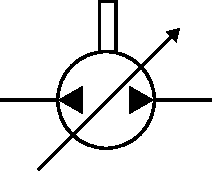
\includegraphics{gfx/writingadvancedcomponents/variablepump.pdf}};
\node[yshift=5pt] () {$D$};
\node[yshift=-20pt, xshift=3pt] () {$C_{leak}$};
\node[yshift=33pt, xshift=40pt] () {$\varepsilon$};
\node[yshift=50pt, xshift=1pt] () {$n$};
\node[yshift=-7pt, xshift=-60pt] () {$p_{1}$};
\node[yshift=-7pt, xshift=60pt] () {$p_{2}$};
\node[xshift=36pt] () {$q$};
\draw[very thick, ->] (25pt,-7pt) -> (44pt,-7pt);
\end{tikzpicture}

\subsection*{Equations}
The flow from a hydraulic pump can be modelled with the following equations:

\begin{equation*}
\begin{cases}
q - q_{leak} = \varepsilon D \omega/2\pi \\
q_{leak} = C_{leak}\Delta p
\end{cases}
\end{equation*}

\noindent Here $q$ is the generated flow and $q_{leak}$ the leakage flow. $\Delta p$ is the pressure difference over the pump. In Hopsan we will have one flow and pressure at each port. Thus, we need to introduce the variables $p_{1}$ and $q_{1}$ for the inlet port, and $p_{2}$ and $q_{2}$ for the outlet. Flow is always defined as positive outwards from Q-type components. Therefore, the inlet flow will be the same as the outlet flow but negative. The equations now become:

\begin{equation*}
\begin{cases}
q_{2} - C_{leak}(p_{1}-p_{2}) = \varepsilon D \omega/2\pi \\
q_{1} = -q_{2}
\end{cases}
\end{equation*}

\noindent However, Hopsan uses the transmission line element method. For this reason we will not get the pressure variables as explicit input variables. Instead, we get a \textit{wave variable} and an \textit{impedance}. The TLM equations are then used to calculate the pressures from the flow variables, according to the two new equations below:

\begin{equation*}
\begin{cases}
q_{2} - C_{leak}(p_{1}-p_{2}) = \varepsilon D \omega/2\pi \\
q_{1} = -q_{2}\\
p_{1} = c_{1} + q_{1}Z_{c,1}\\
p_{2} = c_{2} + q_{2}Z_{c,2}
\end{cases}
\end{equation*}

\noindent It is now possible to rearrange the equations so that the can be solved analytically. First we replace the pressure variables in the first equation with the TLM equations:

\begin{equation*}
\begin{cases}
q_{2} - C_{leak}(c_{1} - q_{2}Z_{c,1}-c_{2} - q_{2}Z_{c,2}) = \varepsilon D \omega/2\pi \\
q_{1} = -q_{2}\\
p_{1} = c_{1} + q_{1}Z_{c,1}\\
p_{2} = c_{2} + q_{2}Z_{c,2}
\end{cases}
\end{equation*}

\noindent Finally, we rearrange the first equation to break out the flow variable:

\begin{equation*}
\begin{cases}
q_{2} = (\varepsilon D \omega/2\pi - C_{leak}(c_{1} -c_{2})) / (1-C_{leak}(Z_{c,1}-Z_{c,2}))\\
q_{1} = -q_{2}\\
p_{1} = c_{1} + q_{1}Z_{c,1}\\
p_{2} = c_{2} + q_{2}Z_{c,2}
\end{cases}
\end{equation*}

\noindent We now have a linear equation system that can be solved step-by-step. 

\subsection*{C++ Code}
First, we create the skeleton for the new component, as described in the previous tutorial. We need two hydraulic ports and four input variables ($\omega$, $D_{p}$, $C_{leak}$ and $\varepsilon$). The resulting code for the class members and the creator functions is shown below:

\noindent 
\begin{minipage}{\linewidth}
\begin{lstlisting}[basicstyle=\footnotesize\ttfamily]
#include "ComponentEssentials.h"

namespace hopsan {

class HydraulicFixedDisplacementPump : public ComponentQ
{
private:
    double *mpND_p1, *mpND_q1, *mpND_c1, *mpND_Zc1; 
    double *mpND_p2, *mpND_q2, *mpND_c2, *mpND_Zc2;
    double *mpW, *mpDp, *mpCleak, *mpEps;
    Port *mpP1, *mpP2;

public:
    static Component *Creator()
    {
        return new HydraulicFixedDisplacementPump();
    }
\end{lstlisting}
\end{minipage}

\noindent The only thing needed in the \texttt{configuration()} function is to create ports and input variables:

\begin{minipage}{\linewidth}
\begin{lstlisting}[basicstyle=\footnotesize\ttfamily]
void configure()
{
    mpP1 = addPowerPort("P1", "NodeHydraulic");
    mpP2 = addPowerPort("P2", "NodeHydraulic");

	addInputVariable("eps", "Displacement setting", "", 1.0, &mpEps);
    addInputVariable("w_p", "Angular Velocity", "rad/s", 250.0, &mpW);
    addInputVariable("D_p", "Displacement", "m^3/rev", 0.00005, &mpDp);
    addInputVariable("C_leak", "Leakage Coeff.", "(m^3/s)/Pa", 0.0, &mpCleak);
}
\end{lstlisting}
\end{minipage}

\noindent The \texttt{initialize()} function will only need the \texttt{getSafeDataNodePtr()} function calls:

\begin{minipage}{\linewidth}
\begin{lstlisting}[basicstyle=\footnotesize\ttfamily]
void initialize()
{
    mpND_p1 = getSafeNodeDataPtr(mpP1, NodeHydraulic::Pressure);
    mpND_q1 = getSafeNodeDataPtr(mpP1, NodeHydraulic::Flow);
    mpND_c1 = getSafeNodeDataPtr(mpP1, NodeHydraulic::WaveVariable);
    mpND_Zc1 = getSafeNodeDataPtr(mpP1, NodeHydraulic::CharImpedance);

    mpND_p2 = getSafeNodeDataPtr(mpP2, NodeHydraulic::Pressure);
    mpND_q2 = getSafeNodeDataPtr(mpP2, NodeHydraulic::Flow);
    mpND_c2 = getSafeNodeDataPtr(mpP2, NodeHydraulic::WaveVariable);
    mpND_Zc2 = getSafeNodeDataPtr(mpP2, NodeHydraulic::CharImpedance);
}
\end{lstlisting}
\end{minipage}

\noindent Now it is time for the interesting part, to write the actual equations in the \texttt{simulateOneTimestep()} function. The final code is presented below. Some of the steps below will already be done if you used HoLC to generate the code.

\begin{tutenumerate}
\tutitem{Create local variables}
We begin with creating local variables for the port variables (line 3-4 below).

\tutitem{Read input variables} 
Assign all input variables them with their corresponding pointers (line 6-16).

\tutitem{Write the pump equations}
The equations must be converted to C++ syntax (line 18-22).

\tutitem{Check for cavitation}
In order to make the model physically correct, we must make sure that negative pressures are not allowed. For this we create a boolean variable for cavitation and assign it with false (line 25). Then we check if pressure $p_{1}$ or $p_{2}$ is smaller than zero. If they are, we set the cavitation boolean to true and assign $c_{1}$ and $Z_{c,1}$ with zero (line 26-37).

\tutitem{Handle the cavitation}
If the cavitation boolean is true, at least one of the pressures was negative. In this case we need to recalculate the flow and the pressure variables (line 39-46). 

\tutitem{Write output variables}
Finally, the output variables must be written to the nodes (line 48-52).

\end{tutenumerate}

\begin{minipage}{\linewidth}
\begin{lstlisting}[basicstyle=\footnotesize\ttfamily]
void simulateOneTimestep()
{
    //Declare local variables
    double p1, q1, c1, Zc1, p2, q2, c2, Zc2, w, dp, Cleak, eps;

    //Read input variables
    w = (*mpW);
    dp = (*mpDp);
    Cleak = (*mpCleak);
    eps = (*mpEps);

    //Get variable values from nodes
    c1 = (*mpND_c1);
    Zc1 = (*mpND_Zc1);
    c2 = (*mpND_c2);
    Zc2 = (*mpND_Zc2);

    //Fixed Displacement Pump equations
    q2 = ( dp*eps*w/(2.0*pi) + Cleak*(c1-c2) ) / ( (Zc1+Zc2)*Cleak+1 );
    q1 = -q2;
    p1 = c1 + Zc1*q1;
    p2 = c2 + Zc2*q2;

    //Check for cavitation
    bool cav = false;
    if (p1 < 0.0)
    {
        c1 = 0.0;
        Zc1 = 0.0;
        cav = true;
    }
    if (p2 < 0.0)
    {
        c2 = 0.0;
        Zc2 = 0.0;
        cav = true;
    }
    
    //Handle cavitation
    if (cav)
    {
        q2 = ( dp*eps*w/(2.0*pi) + Cleak*(c1-c2) ) / ( (Zc1+Zc2)*Cleak+1 );
		q1 = -q2;
        p1 = c1 + Zc1 * q1;
        p2 = c2 + Zc2 * q2;
    }

    //Write new values to nodes
    (*mpND_p1) = p1;
    (*mpND_q1) = q1;
    (*mpND_p2) = p2;
    (*mpND_q2) = q2;
}
\end{lstlisting}
\end{minipage}

\vfill

\section*{Translational Mass}
This part of the tutorial will explain how to write a translational mass component with second order dynamics. It will contain a mass and a damping coefficient, as shown in the figure below. We leave out dry friction and spring coefficient for simplicity.

\begin{tikzpicture}
\node[] () {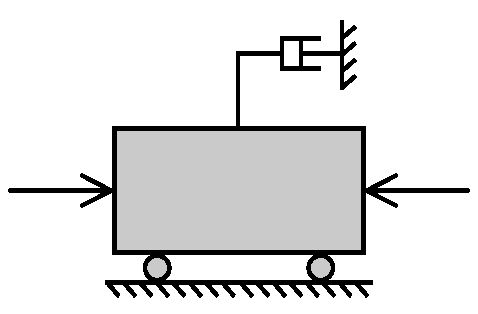
\includegraphics[width=6cm]{gfx/writingadvancedcomponents/mass.pdf}};
\node[yshift=-10pt, xshift=0pt] () {$M$};
\node[yshift=-3pt, xshift=-70pt] () {$F_{1}$};
\node[yshift=-3pt, xshift=70pt] () {$F_{2}$};
\node[yshift=36pt, xshift=55pt] () {$B$};
\end{tikzpicture}

\subsection*{Equations}

The fundamental equation in the component will be Newton's second law of motion:

\begin{equation*}
M\ddot{x} + B\dot{x} = \sum{F}
\end{equation*}

\noindent The Hopsan component will have two ports, which will be defined in opposite directions. It is also necessary to provide equivalent mass variables, which are required by some other components in Hopsan:

\begin{equation*}
\begin{cases}
M\ddot{x_{2}} + B\dot{x_{2}} = F_{1} - F_{2}\\
x_{1} = -x_{2} \\
\dot{x}_{1} = -\dot{x}_{2} \\
m_{e,1} = M \\
m_{e,2} = M
\end{cases}
\end{equation*}

\noindent Finally, we must add the TLM equations in order to calculate the force from the wave variables and impedances:

\begin{equation*}
\begin{cases}
M\ddot{x_{2}} + B\dot{x_{2}} = F_{1} - F_{2}\\
x_{1} = -x_{2} \\
\dot{x}_{1} = -\dot{x}_{2} \\
m_{e,1} = M \\
m_{e,2} = M \\
F_{1} = c_{1} + Z_{c,1}\dot{x}_{1} \\
F_{2} = c_{2} + Z_{c,2}\dot{x}_{2} 
\end{cases}
\end{equation*}

\noindent The equations of the mass is more complicated than the ones for the pump, since it contains time derivatives ($ddot{x}$ and $dot{x}$). Hopsan uses bilinear transforms to solve such equations. In order to use these, we must convert the first equation into a Laplace transform. We use a first order transform to calculate the velocity. Then the position can be obtained by integrating the velocity. By adding the impedance directly to the damping, we can use the wave variables as the external force. In this way we can calculate $x$ and $v$ without first calculating the forces. 

\begin{equation*}
\begin{cases}
v_{2} = \dfrac{1}{M s + B}(F_{1}-F_{2}) = \dfrac{1}{M s + (B+Z_{c,1}+Z_{c,2})}(c_{1}-c_{2}) \\
\dot{x}_{2} = v_{2} \\
v_{1} = -v_{2} \\
x_{1} = -x_{2} \\
F_{1} = c_{1} + Z_{c,1}v_{1} \\
F_{2} = c_{2} + Z_{c,2}v_{2} 
\end{cases}
\end{equation*}

\subsection*{C++ Code}
As with the previous component, we begin by creating a code skeleton. We want two mechanical ports, a constant parameter for the mass and input variables for damping and minimum and maximum position. Note that we also need to include the file \texttt{ComponentUtilities.h}, which contain classes for the transfer function and the integration.
 	
\noindent 
\begin{minipage}{\linewidth}
\begin{lstlisting}[language=c++, basicstyle=\footnotesize\ttfamily]
#include "ComponentEssentials.h"
#include "ComponentUtilities.h"

namespace hopsan {

class MechanicTranslationalMass : public ComponentQ
{
private:
    Port *mpP1, *mpP2;
    double *mpP1_f, *mpP1_x, *mpP1_v, *mpP1_c, *mpP1_Zc, *mpP1_me;
    double *mpP2_f, *mpP2_x, *mpP2_v, *mpP2_c, *mpP2_Zc, *mpP2_me;
    double *mpB, *mpXMin, *mpXMax;
    double mMass;

    FirstOrderTransferFunction mTF;
    Integrator mIntegrator;
    double mNum[2], mDen[2];

public:
    static Component *Creator()
    {
        return new MechanicTranslationalMass();
    }
\end{lstlisting}
\end{minipage}
 	
\noindent There is nothing special with the \texttt{configure()} function. All we need to do here is to create the ports, the constant and the input variables.

\noindent 
\begin{minipage}{\linewidth}
\begin{lstlisting}[basicstyle=\footnotesize\ttfamily]
void configure()
{
    mpP1 = addPowerPort("P1", "NodeMechanic");
    mpP2 = addPowerPort("P2", "NodeMechanic");

    addConstant("m",          "Mass",               "kg",   100.0, mMass);
    
    addInputVariable("B",     "Viscous Friction",   "Ns/m", 10.0,  &mpB);
    addInputVariable("x_min", "Minimum Position",   "m",    0.0,   &mpXMin);
    addInputVariable("x_max", "Maximum Position",   "m",    1.0,   &mpXMax);
}
\end{lstlisting}
\end{minipage}
 
\noindent The \texttt{initialize()} function is a little more advanced than for the pump. We need to initialize the transfer function and the integrator with start values for $f$, $v$ and $x$. We also need to define the coefficients for the transfer function. This is done with two arrays called \texttt{mDen} and \texttt{mNum}, according to this:\\

$\dfrac{mNum[1] s + mNum[0]}{mDen[1] s + mNum[0]}$\\
 
 
\noindent Finally, we also need to initialize the equivalent mass variables in the nodes.

\noindent 
\begin{minipage}{\linewidth}
\begin{lstlisting}[basicstyle=\footnotesize\ttfamily]
void initialize()
{
    mpP1_f = getSafeNodeDataPtr(mpP1, NodeMechanic::Force);
    mpP1_x = getSafeNodeDataPtr(mpP1, NodeMechanic::Position);
    mpP1_v = getSafeNodeDataPtr(mpP1, NodeMechanic::Velocity);
    mpP1_c = getSafeNodeDataPtr(mpP1, NodeMechanic::WaveVariable);
    mpP1_Zc = getSafeNodeDataPtr(mpP1, NodeMechanic::CharImpedance);
    mpP1_me = getSafeNodeDataPtr(mpP1, NodeMechanic::EquivalentMass);

    mpP2_f = getSafeNodeDataPtr(mpP2, NodeMechanic::Force);
    mpP2_x = getSafeNodeDataPtr(mpP2, NodeMechanic::Position);
    mpP2_v = getSafeNodeDataPtr(mpP2, NodeMechanic::Velocity);
    mpP2_c = getSafeNodeDataPtr(mpP2, NodeMechanic::WaveVariable);
    mpP2_Zc = getSafeNodeDataPtr(mpP2, NodeMechanic::CharImpedance);
    mpP2_me = getSafeNodeDataPtr(mpP2, NodeMechanic::EquivalentMass);

    //Read node variables
    double f1, f2, x2, v2;
    f1 = (*mpP1_f);
    f2 = (*mpP2_f);
    x2 = (*mpP2_x);
    v2 = (*mpP2_v);

    //Initialization code
    mNum[0] = 1.0;
    mNum[1] = 0.0;
    mDen[0] = (*mpB);
    mDen[1] = mMass;

    mTF.initialize(mTimestep, mNum, mDen, f1-f2, v2);
    mIntegrator.initialize(mTimestep, x2, v2); 
    
    //Write values to nodes
    (*mpP1_me) = mMass;
    (*mpP2_me) = mMass;
}
\end{lstlisting}
\end{minipage}
 	
 	
\noindent Last but not least, we need to write the \texttt{simulateOneTimeStep()} function. This is explained step-by-step: 
\begin{tutenumerate}
\tutitem{Define local variables}
Define local variables for input variables and node values (line 3-4)
\tutitem{Read from input variables}
Assign input variables to local variables (line 6-9)
\tutitem{Read from nodes}
Assign node variables to local variables (line 11-15)
\tutitem{Update the damping coefficient}
Update the coefficient in the transfer function by adding the impedance variables to the damping factor (line 17-19)
\tutitem{Calculate velocity}
Use the transfer function to calculate $v_{2}$ from $c_{1}-c_{2}$ (line 21-22)
\tutitem{Calculate position}
Use the integrator to calculate $x_{2}$ as a function of $v_{2}$ (line 24-25)
\tutitem{Handle limitations}
Reset variables and re-initialize the transfer function and the integrator if $x_{2}$ is outside limits (line 27-41)
\tutitem{Calculate the remaining variables}
Calulate velocity and position for node 1 ($v_{1}$, $x_{1}$), and then calculate, $F_{1}$ and $F_{2}$ using the TLM equations (line 43-47)
\tutitem{Write values to the nodes}
Write back the values of the local variables to the node variables (line 49-57)
\end{tutenumerate}
 	
\noindent 
\begin{minipage}{\linewidth}
\begin{lstlisting}[basicstyle=\footnotesize\ttfamily] 	
void simulateOneTimestep()
{
    //Declare local variables
    double f1, x1, v1, c1, Zc1, f2, x2, v2, c2, Zc2, B, xmin, xmax;

    //Read input variables
    B = (*mpB);
    xmin = (*mpXMin);
    xmax = (*mpXMax);
            
    //Get variable values from nodes
    c1 = (*mpP1_c);
    Zc1 = (*mpP1_Zc);
    c2 = (*mpP2_c);
    Zc2 = (*mpP2_Zc);

    //Mass equations
    mDen[0] = B+Zc1+Zc2;
    mTF.setDen(mDen);

    //Calculate velocity
    v2 = mTF.update(c1-c2);
    
    //Calculate position
    x2 = mIntegrator.update(v2);

    //Handle position limits
    if(x2<xmin)
    {
        x2=xmin;
        v2=0.0;
        mTF.initializeValues(c1-c2, v2);
        mIntegrator.initializeValues(v2, xmin);
    }
    if(x2>xmax)
    {
        x2=xmax;
        v2=0.0;
        mTF.initializeValues(c1-c2, v2);
        mIntegrator.initializeValues(v2, xmax);
    }

    //Calculate remainig varaibles
    v1 = -v2;
    x1 = -x2;
    f1 = c1 + Zc1*v1;
    f2 = c2 + Zc2*v2;

    //Write new values to nodes
    (*mpP1_f) = f1;
    (*mpP1_x) = x1;
    (*mpP1_v) = v1;
    (*mpP2_f) = f2;
    (*mpP2_x) = x2;
    (*mpP2_v) = v2;
    (*mpP1_me) = mMass;
    (*mpP2_me) = mMass;
}
\end{lstlisting}
\end{minipage}
 
\end{document}
